%%%%%%%%%%%%%%%%%%%%%%%%%%%%%%%%%%%%%%%%%%%%%%%%%%%%%%%%%%%%%%%%%%%%%%%%
\chapter{State of the Art}
\label{sec:stateOfTheArt}
%%%%%%%%%%%%%%%%%%%%%%%%%%%%%%%%%%%%%%%%%%%%%%%%%%%%%%%%%%%%%%%%%%%%%%%%

Um Rest Frameworks für die Evaluierung zu finden, wurde eine Technologierecherche durchgeführt. Dabei konnten folgende Projekte gefunden werden, welche eine REST-Anbindung für Android unterstützen:
\begin{itemize}
	\item Resty (\href{http://beders.github.io/Resty/Resty/Overview.html}{http://beders.github.io/Resty/Resty/Overview.html})
	\item Retrofit (\href{http://square.github.io/retrofit/}{http://square.github.io/retrofit/})
	\item RESTlet (\href{http://restlet.com/}{http://restlet.com/})
	\item Spring for Android (\href{http://projects.spring.io/spring-android/}{http://projects.spring.io/spring-android/})
	\item CRest (\href{http://crest.codegist.org/index.html}{http://crest.codegist.org/index.html})
	\item RESTeasy Mobile (\href{http://resteasy.jboss.org/}{http://resteasy.jboss.org/})
	\item RESTDroid (\href{http://pcreations.fr/me/restdroid-resource-oriented-rest-client-for-android}{http://pcreations.fr/me/restdroid-resource-oriented-rest-client-for-android})
	\item Jersey (\href{https://jersey.java.net/}{https://jersey.java.net/})
\end{itemize}

Es würde den Rahmen der Bachelorarbeit überschreiten, all diese gefundenen REST Frameworks zu evaluieren. Daher wurde einer Vorstudie gemacht, aufgrund derer die drei populärsten und den Anforderungen adäquatesten Frameworks ausgewählt wurden.
\\\\
Die Popularität eines Frameworks gibt eine gewisse Auskunft über die Qualität, da für diese Frameworks oft besserer Support in Form von Dokumentation, sowie eine größere und aktivere Community zur Verfügung steht. Eine Studie von Chris Parnin\cite{parnin2012crowd} beschäftigt sich damit, wie "'Crowd documentation"' beispielsweise auf \acrfull{QA} Webseiten, die Hilfestellung zu verschiedenen Frameworks beeinflusst. Verwenden viele Entwickler ein Framework, sind dadurch mehr Fragen auf Q\&A Webseiten vorhanden und dadurch können mögliche Fragen besser beantwortet werden. Durch eine Erhebung der Anzahl von Fragen auf Stack Overflow\footnote{\href{http://stackoverflow.com/}{http://stackoverflow.com/}} und der Stars auf GitHub\footnote{\href{https://github.com/}{https://github.com/}} wurden Rückschlüsse auf die Popularität der einzelnen Frameworks gezogen.  
\\\\
In dem Artikel "'How to identify a strong open source project"\cite{balter:strongOS} werden verschiedene Indikatoren erhoben, welche Rückschlüsse auf eine solide und gute Entwicklung eines Frameworks geben. Deswegen wurden zusätzlich noch verschiedene Aktivitäten auf GitHub verglichen, wie Datum des letzten Commits, oder die Anzahl der Commits.

\begin{minipage}{\textwidth} 
	\centering	
	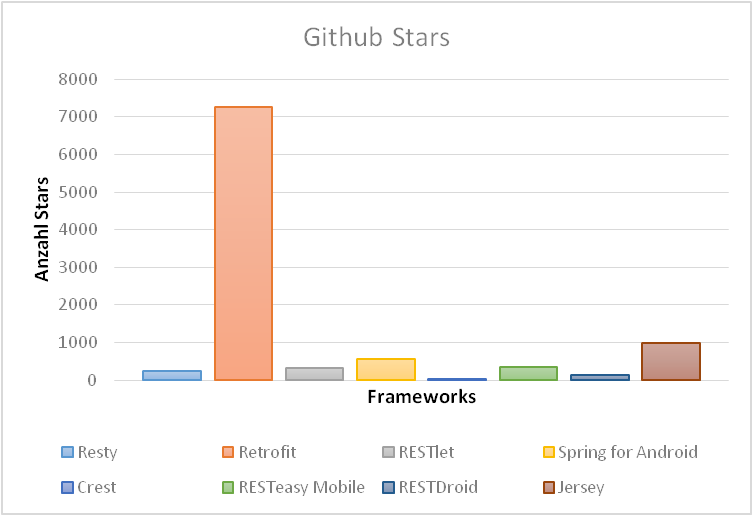
\includegraphics[width=0.60\textwidth]{figures/github_stars.png}
	\captionof{figure}{Github Stars, aktualisiert am 01.03.2016}
	\label{figure:githubStars}
	\vspace{2ex}
\end{minipage}

\begin{minipage}{\textwidth} 
	\centering	
	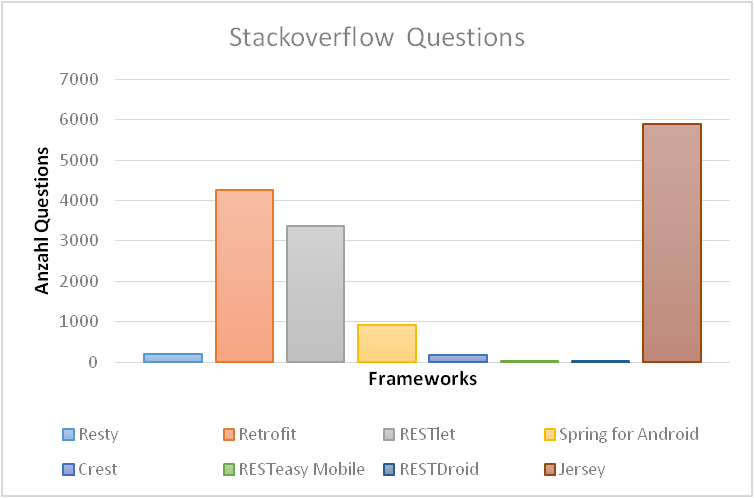
\includegraphics[width=0.60\textwidth]{figures/stackoverflow_questions.png}
	\captionof{figure}{Stackoverflow Questions, aktualisiert am 01.03.2016}	
	\label{figure:stackoverflowQuestions}
	\vspace{2ex}
\end{minipage}

\begin{minipage}{\textwidth} 
	\centering	
	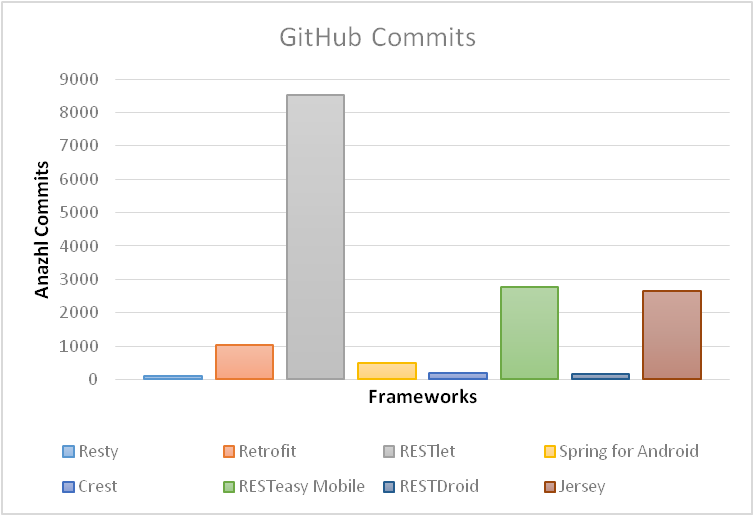
\includegraphics[width=0.60\textwidth]{figures/github_commits.png}
	\captionof{figure}{Github Commits, aktualisiert am 01.03.2016}	
	\label{figure:githubCommits}
	\vspace{2ex}
\end{minipage}

\begin{minipage}{\textwidth} 
	\centering	
	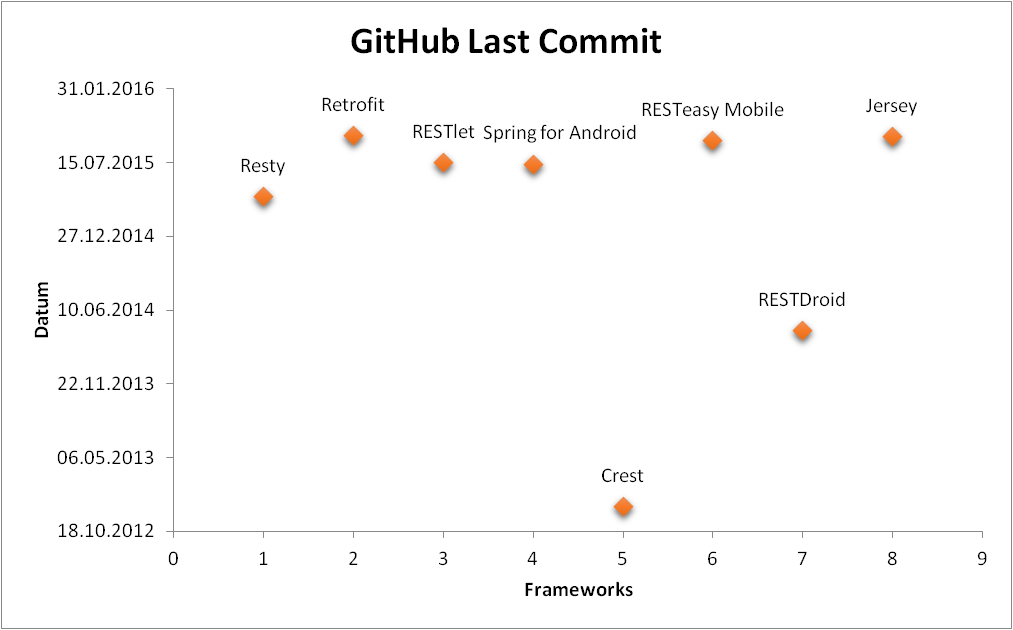
\includegraphics[width=0.65\textwidth]{figures/github_lastCommit.png}
	\captionof{figure}{GitHub Last Commit, aktualisiert am 01.03.2016}	
	\label{figure:githubLastCommit}
	\vspace{5ex}
\end{minipage}

Aufgrund der Vorstudie werden folgende REST-Frameworks evaluiert und miteinander verglichen:

\begin{itemize}
	\item AndroidAnnotations
	\item Jersey
	\item Retrofit 	
	\item Spring for Android
\end{itemize}
